% DIVAS image processing workshop
% OpenCV images slides
%
% Mark M. Meysenburg
% 5/14/2017

\documentclass{beamer}

\mode<presentation> {

% set theme and color
\usetheme{CambridgeUS}
\usecolortheme{crane}
}

\usepackage{graphicx} % Allows including images

\usepackage{listings} % Allow sourcecode

\usepackage{hyperref} % Allow clickable hyperlinks

%----------------------------------------------------------------------------------------
%	TITLE PAGE AND FRONT MATTER
%----------------------------------------------------------------------------------------

\title[Image Basics]{IP Workshop: OpenCV Images} % The short title appears at the bottom of every slide, the full title is only on the title page

\author{Mark M. Meysenburg} % Your name
\institute[Doane DIVAS] % Your institution as it will appear on the bottom of every slide, may be shorthand to save space
{
Doane University \\ % Your institution for the title page
\medskip
\textit{mark.meysenburg@doane.edu} % Your email address
}
\date{\today} % Date, can be changed to a custom date

\begin{document}

\lstset{basicstyle=\footnotesize,language=Python}

\begin{frame}
\titlepage % Print the title page as the first slide
\end{frame}

\begin{frame}
\frametitle{Overview} 
\tableofcontents 
\end{frame}

%----------------------------------------------------------------------------------------
%	PRESENTATION SLIDES
%----------------------------------------------------------------------------------------

\section{Images / Arrays}

\begin{frame}
	\frametitle{OpenCV images are NumPy arrays}

	\begin{itemize}

		\item OpenCV images are stored in a manner consistent with our raster graphics model

		\begin{itemize}

			\item An image is rectangular array of pixels

			\item Each pixel has three color channel values (RGB)

		\end{itemize}

		\item OpenCV images = 3D NumPy arrays

		\item Remember the coordinate system, and think BGR vs. RGB
	\end{itemize}

\end{frame}

\begin{frame}
	\frametitle{OpenCV images are NumPy arrays}

	\begin{center}
		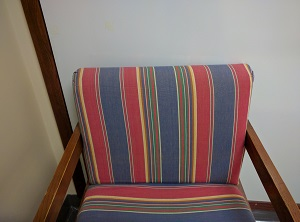
\includegraphics[width=0.75\textwidth]{../../fig/02-chair-orig.jpg}
	\end{center}

\end{frame}

\begin{frame}
	\frametitle{OpenCV images are NumPy arrays}

	\begin{center}
		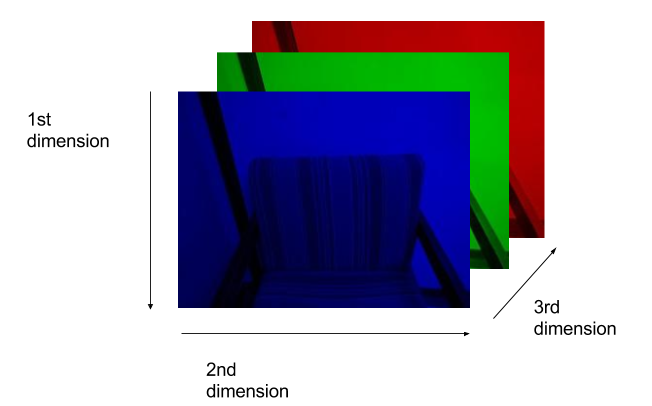
\includegraphics[width=0.75\textwidth]{../../fig/02-chair-layers.png}

	\end{center}

\end{frame}

\section{Image I/O}

\begin{frame}
	\frametitle{Reading, displaying, saving}

	\begin{itemize}
		\item OpenCV has methods for reading, displaying, and saving images

		\item All popular formats supported

		\item In Python programs, we gain access to the OpenCV library via the \lstinline!import cv2! statement

	\end{itemize}

\end{frame}

\begin{frame}
	\frametitle{Reading, displayng, saving}

	See the {\tt Workshops/image-processing/02-opencv-images/Open.py} program for examples of reading, displaying, and saving images.

	Key methods:

	\begin{itemize}

		\item \lstinline!cv2.imread()!

		\item \lstinline!cv2.namedWindow()!

		\item \lstinline!cv2.imshow()!

		\item \lstinline!cv2.waitKey()!

		\item \lstinline!cv2.imwrite()!

	\end{itemize}
\end{frame}

\end{document}


